\myChapter{Appendix: OSGi}\label{chap:appendixosgi}
\minitoc\mtcskip
\vfill
\section{OSGi Architecture}
To understand how OSGi \cite{Moussa2010ServiceComposition} works and which capabilities could offer to the EA practitioners it is necessary to understand how OSGi is built. OSGi has a layered model that is depicted in Figure \ref{fig:osgi-original}. The terms present in this figure are:

\begin{itemize}
\item Bundles: OSGi components made by developers. They are a normal {\em jar} file including Java classes, interfaces and extra files (such as the {\em Service Descriptions}). They also have additions to the MANIFEST.MF file (a metadata file with information about the {\em jars}).
\item Services: This layer connects bundles in a dynamic way by offering a publish-find-bind model.
\item Life-Cycle: The API to install, start, stop, update, and uninstall bundles.
\item Modules: This layer defines how a bundle can import and export code (using the MANIFEST.MF file).
\item Security: Security aspects are handled in this layer.
\item Execution Environment: Defines what methods and classes are available in a specific platform. For example, mobile devices have less Java classes due to performance constraints.
\end{itemize}

\begin{SCfigure}[20][tb]
\centering
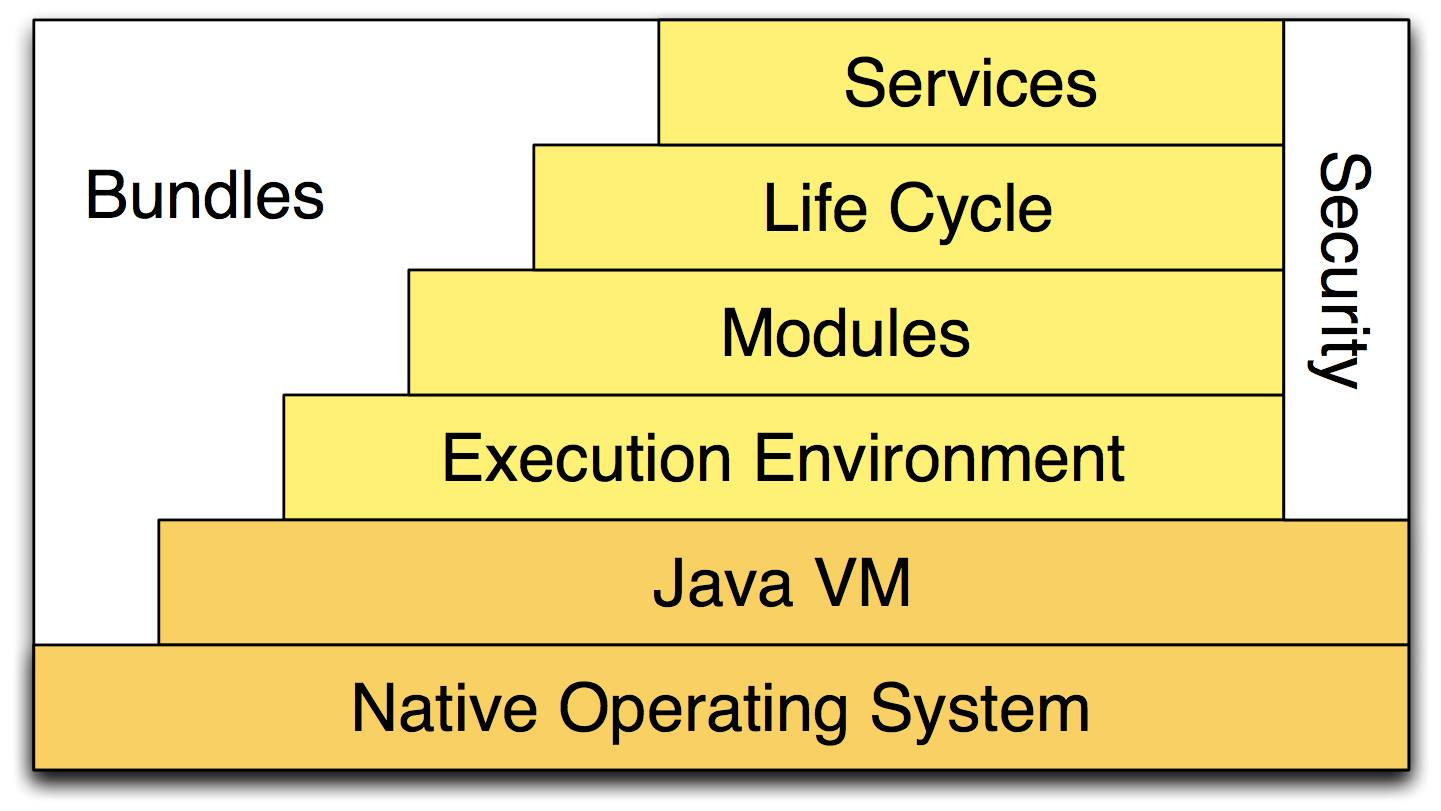
\includegraphics[width=26pc]{gfx/soa/osgi-oficial.jpg}
\caption{OSGi layered architecture. Every layer is built from the one just below.}
\label{fig:osgi-original}
\end{SCfigure}






\section{OSGi configuration files}
With respect to the OSGi layers introduced above, this section details how to use all OSGi capabilities. 

OSGi implements a dynamic component model, unlike normal Java
environments. Applications or components (also called
\emph{bundles}) can be remotely installed, started, stopped, updated
or uninstalled on the fly; moreover, the classes and
packaging management is specified in detail. The OSGi framework provides
APIs for the management of services that are exposed or used by the
bundles.

A {\em bundle} is a file containing compiled and packaged classes and a configuration file. This file indicates which classes are importe or exported by the bundle. Being SOA, the most important concept in OSGi is the {\em service}. Services allow {\em bundles} to be dinamically connected, offering a publication-search-connection model. That is, a {\em bundle} exposes a service by a Java interface (service interface in Figure \ref{fig:soadiagram}), and another bundle (or itself) implements that interface. A third {\em bundle} can access this service using the exposed interface without having any knowledge of how it is implemented, using the {\em service registry} (equivalent to service broker of Figure \ref{fig:soadiagram}). Figure \ref{OSGIDIAGRAM} shows an example of the OSGi architecture.


\begin{SCfigure}[20][tb]
\centering
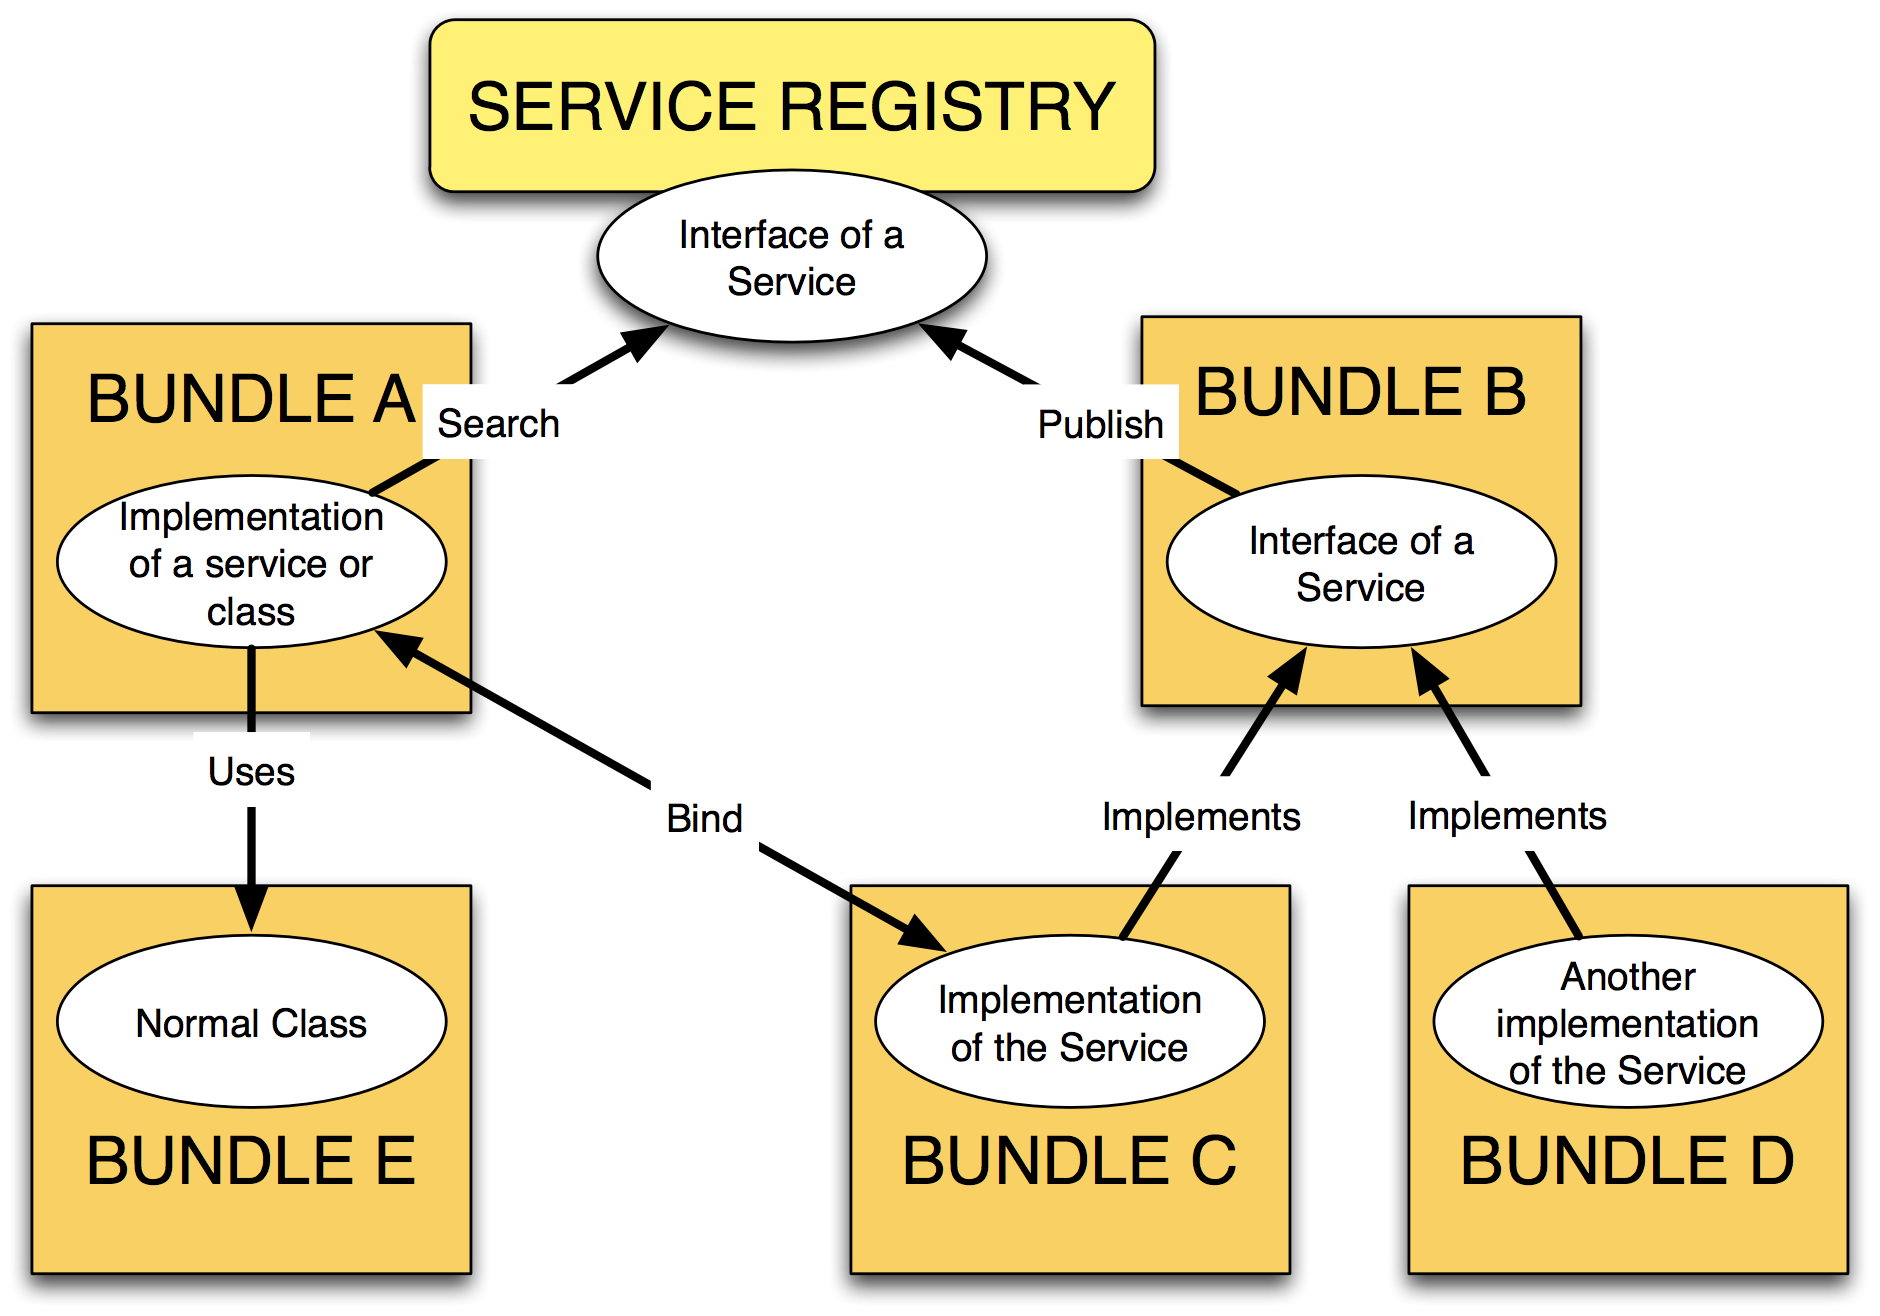
\includegraphics[width=26pc]{gfx/soa/bundles.jpg}
\caption{In OSGi, a service can be implemented by several bundles. Other bundles may chose among this implementations using the service registry. In this figure, Bundles C and D implement a service, and A uses the service registry to use one of them.}
\label{OSGIDIAGRAM}
\end{SCfigure}



Java programmers are familiar with the {\em jar} concept. The first difference among a {\em bundle} and a {\em jar} is that the first one has a MANIFEST.MF file adapted to be used in OSGi. This file indicates which classes imports or exports the {\em bundle}. An example can be seen in Figure \ref{fig:manifest}. This file shows the name of the bundle and its version (this is useful to select specific services), and the execution environment (that is, the Java Virtual Machine required). Also, this file specifies the XML files of the declarative services (in section {\em Service-Component}). However, this {\em bundle} can be used as a normal {\em jar} outside OSGi.

\begin{SCfigure}[20][tb]
\noindent
\ttfamily \footnotesize
\hlstd{}{\bf Manifest-Version:} 1.0\\
\hlstd{}{\bf Bundle-ManifestVersion:} 2\\
\hlstd{}{\bf Bundle-Name:} VRP\\
\hlstd{}{\bf Bundle-SymbolicName:} VRP\\
\hlstd{}{\bf Bundle-Version:} 1.0.0\\
\hlstd{}{\bf Bundle-RequiredExecutionEnvironment:} JAVA-1.6\\
\hlstd{}{\bf Import-Package:}  es.ugr.osgiliath,\\
 \hlstd{}  es.ugr.osgiliath.algorithms,\\
\hlstd{} es.ugr.osgiliath.events,\\
 \hlstd{}es.ugr.osgiliath.evolutionary,\\
 \hlstd{}es.ugr.osgiliath.evolutionary.basiccomponents.genomes,\\
 \hlstd{}es.ugr.osgiliath.evolutionary.basiccomponents.individuals,\\
 \hlstd{}es.ugr.osgiliath.evolutionary.elements,\\
 \hlstd{}es.ugr.osgiliath.evolutionary.individual,\\
 \hlstd{}es.ugr.osgiliath.evolutionary.migrator,\\
 \hlstd{}es.ugr.osgiliath.geneticalgorithm.distributed,\\
 \hlstd{}es.ugr.osgiliath.problem\\
\hlstd{}{\bf Export-Package:} es.ugr.osgiliath.vrp,\\
 \hlstd{}es.ugr.osgiliath.vrp.individual\\
\hlstd{}\hlkwa{Service-Component:} OSGI-INF/vrpinitializer.xml,\\
OSGI-INF/vrpfitnesscalculator.xml,\\
 OSGI-INF/vrpcrossover.xml,\\
 OSGI-INF/vrpmutation.xml\\
\mbox{}
 
\normalfont
\caption{Example of MANIFEST.MF. This example defines which packages are necessary to activate the bundle and which packages are exported.}
\label{fig:manifest}
\end {SCfigure}





In normal environments, the creation of a specific implementation of an interface (i.e. {\em FitnessCalculator}) is done as shown in Figure \ref{fig:normalImp}.

\newsavebox{\mintedboxOSGIinst}
\begin{lrbox}{\mintedboxOSGIinst}
\begin{minipage}{10cm}
\begin{minted}[mathescape,
               linenos,
               frame=lines,
               framesep=2mm]{java}
class EvolutionaryAlgorithm implements Algorithm{
 FitnessCalculator fc;
 //A new instance is bound to a reference
 fc = new ExampleFunction();
}
\end{minted}
\end{minipage}
\end{lrbox}

\begin{SCfigure}[20][tb]
\usebox{\mintedboxOSGIinst}
\caption{Normal way to implement an interface in Java.} 
\label{fig:normalImp} 
\end{SCfigure}


With Declarative Services, the \texttt{new ExampleFunction()} part is not used, so if a new implementation is desired no code recompilation is necessary.  Figure \ref{fig:ds} shows a declarative service description file, which establishes in execution time which implementation is bound to the interfaces. This example indicates that the implementation of service \texttt{FitnessCalculator} is \texttt{VRP\-Fit\-ness\-Cal\-cu\-la\-tor}, but this service is not activated until all their references (other services, like \texttt{TransportData}) are also activated. The tag \texttt{cardinality} means that at least one service of that kind must exist (the first \texttt{1} represents optionality) and  the second part (the other \texttt{1} indicates the number of different implementations that can be managed: one (\texttt{1}) or many (\texttt{*}). It is also necessary to create XML files for the rest of services to be exposed (i.e. \texttt{TransportData}) . The file where these capabilities are defined is declared in the section \texttt{Service-Component} of the MANIFEST.MF file, as can be seen in Figure \ref{fig:manifest}.



\newsavebox{\mintedboxOSGIDS}
\begin{lrbox}{\mintedboxOSGIDS}
\begin{minipage}{10cm}
\begin{minted}[linenos,
               fontsize=\scriptsize,
               frame=lines,
               framesep=2mm]{xml}
<?xml version="1.0" encoding="UTF-8"?>
<scr:component xmlns:scr="http://www.osgi.org/xmlns/scr/v1.1.0"
name="VRPFitnessCalculator" >
<implementation class="es.ugr.osgiliath.vrp.VRPFitnessCalculator"/>
<service>
<provide 
interface="es.ugr.osgiliath.evolutionary.elements.FitnessCalculator"/>
</service>
<reference bind="setTransportData"
unbind="unsetTransportData"
cardinality="1..1"
interface="es.ugr.osgiliath.vrp.TransportData"
name="TransportData"
policy="static"
/>
<property name="name" type="String"
value="vrpfitnesscalculator"/>
</scr:component>
\end{minted}
\end{minipage}
\end{lrbox}


\begin{SCfigure}[20][tb]
\usebox{\mintedboxOSGIDS}
\caption{Service Description. This documents indicates that the implementation of the service \texttt{FitnessCalculator} is \texttt{VRPFitnessCalculator}, but it can not activate until their references (other services) are activated.}
\label{fig:ds} 
\end{SCfigure}

Code in Figure \ref{fig:OSGIspecific} shows the code for this implementation.

\newsavebox{\mintedboxOSGIspecific}
\begin{lrbox}{\mintedboxOSGIspecific}
\begin{minipage}{10cm}
\begin{minted}[mathescape,
               linenos,
               fontsize=\footnotesize,
               frame=lines,
               framesep=2mm]{java}
class VRPFitnessCalculator implements FitnessCalculator{
 //Other service references,
 TransportData tdata;
 
 //Methods to bind/unbind each reference
 public TransportData 
    setTransportData(TransportData tdata){
  this.tdata = tdata;
 }
	
 public void 
    unsetTransportData(TransportData tdata){
  this.tdata = null;
 }

 //Implementation of the interface method
 List<Fitness> calculateFitness(List<Individual> inds){
 	...
 }
}
\end{minted}
\end{minipage}
\end{lrbox}

\begin{SCfigure}[20][tb]
\usebox{\mintedboxOSGIspecific}
\caption{Code of the implementation.}
\label{fig:OSGIspecific} 
\end{SCfigure}

%We have to say that in future work these kind of files will be automatically created, being this task transparent to future users of the OSGiLiatH framework.

\section{Event Administration}
The Event Administration in OSGi lets the usage of a blackboard communication architecture where bundles can broadcast or receive events without advertising which bundles are sending or receiving these events.

%Acquire a reference to the EventAdmin OSGi service, it implements the org.osgi.service.event.EventAdmin.
%Pick a topic name for the event and make sure that it follows Topic Naming Conventions mentioned above.
%Fill Event Properties in a dictionary that will be passed as a parameter to the publish method.
%Having the Topic Name and Properties, ready invoke one of the following methods of the Event Admin service: postEvent or sendEvent - while postEvent initiates synchronous delivery of the event, sendEvent initiates asynchronous delivery of the event. So by default, your option should be postEvent method unless you have strict requirements to not continue execution until all handlers of the event handle it.

The steps needed to send events to other bundles are:
\begin{itemize}
\item Acquire a reference to the EventAdmin OSGi service (via Declarative Services, for example).
\item Pick a topic name for the event (for example \texttt{``es\-/ugr\-/os\-gi\-liath\-/al\-go\-rithms\-/end\-ge\-ne\-ra\-tion''})
\item Send the event using the \texttt{postEvent} method of EventAdmin, with the topic plus other desired properties %(poner lo de sincrono/asincrono?)
\end{itemize}

Code to send an event to other bundles is shown in Figure \ref{fig:OSGIpostevent}. The programmer specifies the topic String and optional properties to send to other bundles that are listening. The \texttt{ eventAdmin} variable is a reference to \texttt{``org.osgi.service.event. EventAdmin''} service, obtained via Declarative Services or by hand (not showed).


\newsavebox{\mintedboxOSGIpostevent}
\begin{lrbox}{\mintedboxOSGIpostevent}
\begin{minipage}{10cm}
\begin{minted}[mathescape,
               linenos,
               frame=lines,
               framesep=2mm]{java}
Properties props = new Properties(); //Optional
String topic = 
   "es/ugr/osgiliath/algorithms/endgeneration";
Event evt = new Event(topic,props);
eventAdmin.postEvent(evt);
\end{minted}
\end{minipage}
\end{lrbox}

\begin{SCfigure}[20][tb]
\usebox{\mintedboxOSGIpostevent}
\caption{Code to send an event.}
\label{fig:OSGIpostevent} 
\end{SCfigure}
		
On the other hand, the steps to handle events are:
\begin{itemize}
\item Register a service that implements the OSGi EventHandler interface (via Declarative Services or manually).
\item Specify in this service the topics to subscribe to. For example, the String \texttt{ ``es\-/ugr\-/os\-gi\-li\-ath/al\-go\-ri\-thms/*''} (the * is a wildcard) inside the \texttt{$<$property$>$} tag in the Service Description.
\item Overwrite the handleEvent method of this interface with the desired code.
\end{itemize}

The code  in Figure \ref{fig:OSGIreadevent} shows how to handle events. In this case published the \texttt{ ExampleService} have been published with the implementation \texttt{ ExampleImpl}, that is listening under the topic \texttt{ ``es/ugr/osgiliath/algorithms/*''}.



\newsavebox{\mintedboxOSGIreadevent}
\begin{lrbox}{\mintedboxOSGIreadevent}
\begin{minipage}{10cm}
\begin{minted}[mathescape,
               linenos,
               fontsize=\footnotesize,
               frame=lines,
               framesep=2mm]{java}
class ExampleImpl implements ExampleService,EventHandler{

 public void handleEvent(Event ev){
  if(evt.getTopic().endsWith("endgeneration")){
   // An event with topic 
   // "es/ugr/osgiliath/algorithms
   // /endgeneration"
   System.out.println("Generation over");
  else{
   // Other event with topic starts with
   // "es/ugr/osgiliath/algorithms/"
   System.out.println("Other event received");
  }
 }
}
\end{minted}
\end{minipage}
\end{lrbox}

\begin{SCfigure}[20][tb]
\usebox{\mintedboxOSGIreadevent}
\caption{Code to read an event.}
\label{fig:OSGIreadevent} 
\end{SCfigure}